\documentclass[11pt]{article}

\usepackage[a4paper,margin=2.5cm]{geometry}
\usepackage{microtype}
\usepackage{booktabs}
\usepackage{graphicx}
\usepackage{xcolor}
\usepackage{listings}
\usepackage{enumitem}
\usepackage[colorlinks=true,linkcolor=blue!50!black,urlcolor=blue!50!black]{hyperref}

\definecolor{kw}{RGB}{20,60,140}
\definecolor{codebg}{RGB}{246,246,242}
\definecolor{resbg}{RGB}{242,248,244}

\lstdefinestyle{gl}{
  basicstyle=\ttfamily\small,
  keywordstyle=\bfseries\color{kw},
  backgroundcolor=\color{codebg},
  frame=single, rulecolor=\color{gray!50},
  framesep=5pt, breaklines=true,
  showstringspaces=false, sensitive=true,
  morekeywords={find,follow,group,count,sum,avg,compute,return,limit,budget,tokens,where,order,by,as,assert,edge,merge,distinct,refine,compact,retire,flag,derive,class,from,with,into,prefer,newest,source,reason,continue,same,minus,plus,desc}
}
\lstdefinestyle{res}{
  basicstyle=\ttfamily\small,
  backgroundcolor=\color{resbg},
  frame=single, rulecolor=\color{green!30!gray},
  framesep=5pt, breaklines=true, showstringspaces=false
}

\setlength{\parskip}{4pt}
\setlength{\parindent}{0pt}

\title{\textbf{GraphLang v0: a graph language built for agents,\\ and the engine underneath it}\\[6pt]
\large Project report}
\author{GraphLang project}
\date{August 25, 2026}

\begin{document}
\maketitle

\begin{abstract}
\noindent In one build session we implemented v0 of GraphLang, an agent-optimized graph query and construction language, together with a single-process engine that preserves the architecture of the planned distributed system. We then measured it the only way that matters: head to head against text-to-Cypher on a CypherBench slice, same questions, same models, same retry budget, with the Cypher side executing live on Neo4j. GraphLang with Claude Haiku 4.5 reached 98.3\% execution accuracy against 73.3\% for text-to-Cypher with the same model, and on the multi-hop questions the language was designed around, the gap widened to 96.0\% versus 56.0\%. Every stage of the build passed through an adversarial review loop that surfaced thirteen confirmed defects, all fixed with regression tests before the benchmark numbers were accepted.
\end{abstract}

\section{Why this exists}

When a language model writes a database query today it writes Cypher, SQL, or SPARQL, all designed for people. Frontier models get roughly forty percent of realistic Cypher queries wrong, and they fail in the same few ways every time: they reverse the direction of a relationship arrow, they invent labels the schema does not have, they trip over Cypher's implicit grouping, and they lose track of brackets across long spans. The production world's answer has been to hide the database behind a handful of fixed tools, which works but throws away the ability to ask new kinds of questions.

GraphLang takes the third path: change the language so each of those mistakes is either impossible to write or caught before anything runs. The design decisions were settled in an earlier research phase (eighteen decision points, all documented in the design brief and the spec); this session turned them into working software.

\section{The language, by example}

A query is a short sequence of lines. Each line does one thing and names its result. Here is the flagship example, a multi-hop aggregation over a supply-chain graph:

\begin{lstlisting}[style=gl]
find product where launch_year > 2024 as recent
follow recent uses component as parts
follow parts supplied_by source as sups
group by sups as g
count distinct g.parts as n_parts
return sups.name, n_parts order by n_parts desc budget 2000 tokens
\end{lstlisting}

Four properties of this shape carry the accuracy result. There are no direction arrows: edges are traversed by naming the role you arrive at (\texttt{source}, \texttt{component}), and naming a role your binding already occupies is a type error caught before execution. Every step binds a name, so there is no invisible chaining state to lose track of. Aggregation is staged and explicit: the grouping key lives on its own line and cannot be silently changed by editing the return list, which is the trap that corrupts Cypher aggregations. And the whole program is verified against the live schema before anything executes; a wrong class name comes back as a corrective error with suggestions, ending with the sentence \texttt{nothing was executed.}

The write side is the part no existing query language has. Agents write structurally, with provenance, and every write returns a receipt that carries what changed and any duplicate candidates the write triggered:

\begin{lstlisting}[style=gl]
assert supplier {name: "Ionix Co", country: "KR"}
  source doc:report-08/p1 as ionix
\end{lstlisting}
\begin{lstlisting}[style=res]
receipt: created supplier ionix = #s-1 at @t-1
  guards: schema ok, class invariants ok
  dup candidates: 1
    #s-0954 supplier "Ionix" score 0.97
  resolve with: merge / distinct
\end{lstlisting}

The rest of the surface follows the same pattern: \texttt{merge} and \texttt{distinct} resolve duplicates the system detects; \texttt{refine} splits a coarse blob node into fine-grained children under an agent-supplied mapping, with full lineage back to the source; \texttt{compact} is its inverse; \texttt{retire} invalidates without deleting; \texttt{flag} feeds the per-node health record; and \texttt{derive class} lets agents extend the schema through a gated, provisional path. Health is ordinary queryable data (\texttt{find nodes where health.loss > 0.8}), so graph maintenance is not a special mode, just the same verbs pointed at the graph's own damage report. Results are budgeted in tokens, not rows: overflow truncates cleanly and hands back a continuation token, so a result can never silently flood a context window.

\section{The engine}

The engine is deliberately shaped like the distributed system it will become, shrunk into one process. Durable truth is an append-only write-ahead log plus immutable snapshot runs on disk; memory is rebuilt by replay; nodes are stored with their incident edges so serializing a result is nearly a copy. Positions are monotonic and appear in every receipt. Scaling out later means swapping the storage client for an object-store-backed one, not rewriting the design. Dedup detection runs as a synchronous blocking stage on every write (cheap keys, exact-prefix buckets) plus an asynchronous similarity sweep, feeding a candidate ledger that agents query and resolve. This is the same pipeline shape the full system will use with embeddings; v0 stands the similarity stage in with string ratios.

\section{How it was built: the review loop}

Each implementation stage went through an adversarial review pass by a separate reviewer agent whose brief was to hunt for silent wrong results, not style. The loop was: implement test-first, run the reviewer, fix every confirmed finding with a regression test, re-run the suite, commit. Three rounds produced thirteen confirmed findings. The most serious was a session bug where a binding from an earlier request would pass verification but silently execute against an empty table, returning a well-formed empty result instead of an error; it is exactly the class of failure the language exists to prevent, and it now produces a corrective error instead. The reviewer also caught grammar leaks in the parser (bare words accepted as literals, unbounded column paths), an unfair token-accounting asymmetry in the benchmark harness itself, and a null-comparison hole in the new \texttt{compute} verb. The final suite is 108 tests, all green.

The benchmark was not a one-way measurement; it fed the language. Failure analysis on early passes produced three spec-level changes: aggregates over a plain binding (a whole-result count needs no artificial grouping), per-row edge uniqueness (matching the semantics Cypher uses, so gold answers agree on questions like ``other teams in the same division''), and the \texttt{compute} verb for scalar arithmetic and equality, which the comparison-style questions require. Each change is documented in the spec, and each measurably moved the score.

\section{The benchmark}

The harness draws sixty questions from the CypherBench NBA graph (4{,}327 entities, 18{,}991 relations, loaded identically into the GraphLang engine and into Neo4j 5 running in Docker), stratified across the question categories the v0 language can express. Two conditions run on the identical slice with the identical model and one repair retry each: GraphLang via grammar prompting (a compact tutorial plus worked examples in context; the language has zero training corpus), and text-to-Cypher executing live on Neo4j. Scoring is execution accuracy: normalized, order-insensitive set comparison against CypherBench's published gold answers.

\begin{center}
\begin{tabular}{lrrrrr}
\toprule
Condition & Overall & Multi-hop & 1-hop & Syntax valid & Result tokens \\
\midrule
GraphLang + Haiku 4.5 & \textbf{98.3\%} & \textbf{96.0\%} & \textbf{100\%} & 100\% & 245 \\
text2cypher + Haiku 4.5 & 73.3\% & 56.0\% & 85.7\% & 98.3\% & 394 \\
GraphLang + Sonnet 5 & \textbf{95.0\%} & \textbf{92.0\%} & 97.1\% & 100\% & 278 \\
text2cypher + Sonnet 5 & 71.7\% & 60.0\% & 80.0\% & 96.7\% & 207 \\
\bottomrule
\end{tabular}
\end{center}

For context, the strongest published full-test-set CypherBench numbers are 61.6\% (Claude 3.5 Sonnet) and 60.2\% (GPT-4o); those are on the full benchmark rather than this slice, so they frame rather than directly compare. The cleanest reading of the table is the within-slice, same-model contrast, and its sharpest line is multi-hop with the small model: 96.0\% against 56.0\%. A language with no training data, taught entirely in context, beat the most-documented graph language in the world by forty points exactly where the research predicted a designed language should win, and a small model using GraphLang outperformed a frontier model writing Cypher.

\begin{figure}[h]
\centering
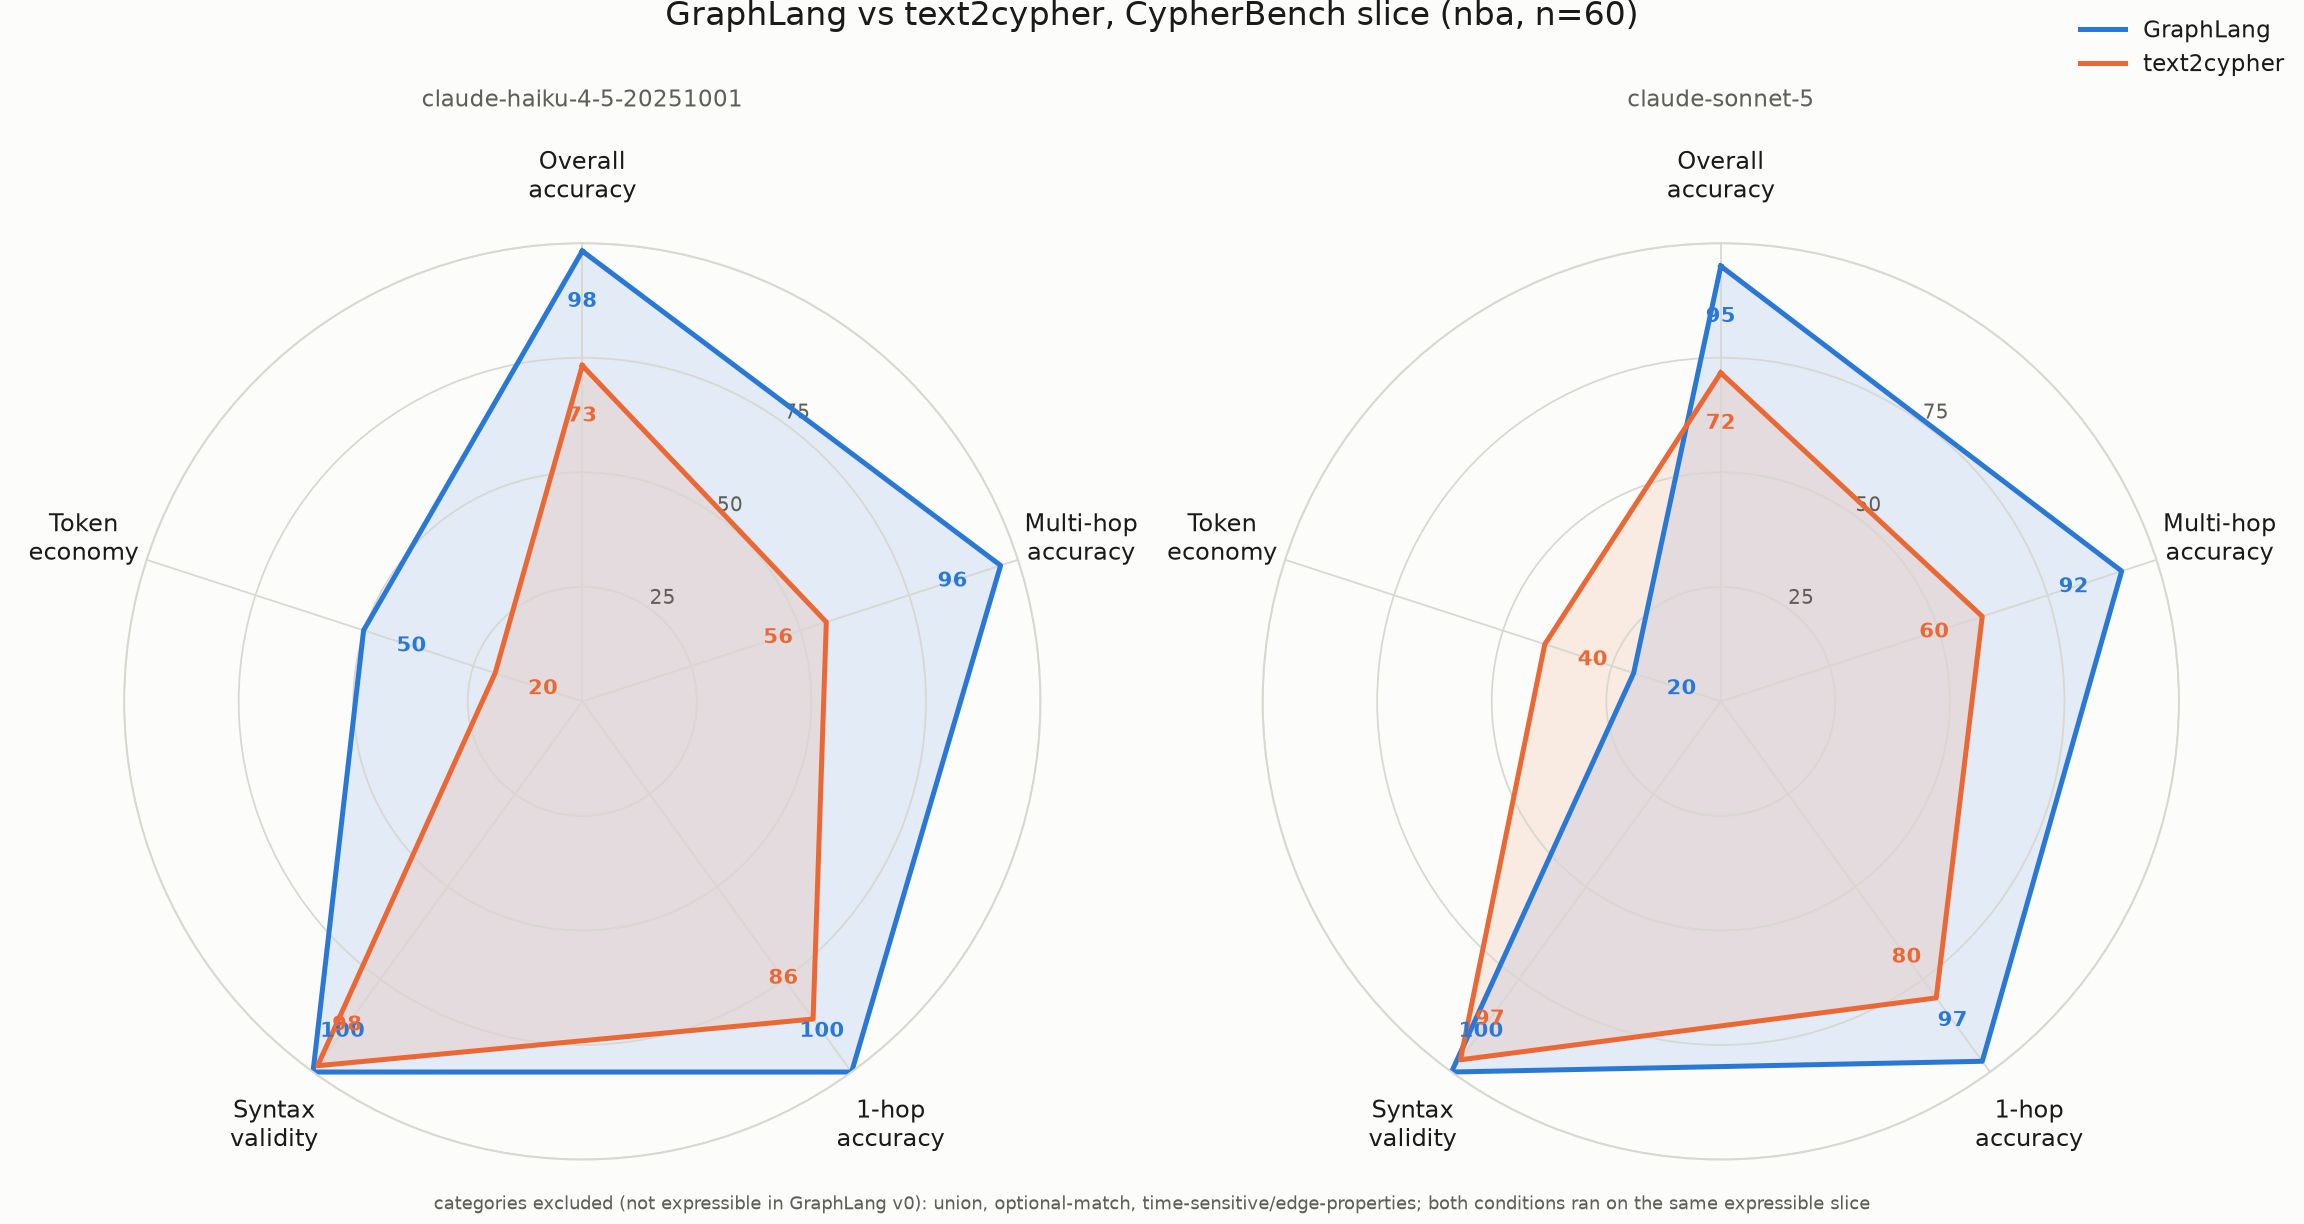
\includegraphics[width=\textwidth]{../../eval/out/spider.png}
\caption{Both conditions, both models, five axes. Token economy is the normalized inverse of mean result tokens.}
\end{figure}

Honesty notes, all also recorded in the results file: the slice covers only categories v0 can express, excluding union, optional-match, and edge-property questions, and both conditions ran on that same slice; it is one domain graph; the two residual GraphLang misses are model discipline errors (an extra return column, a miscounted binding), not engine defects; and on the Sonnet run the Cypher side produced smaller results, so token economy is not uniformly a GraphLang win.

\section{What v0 defers}

Constrained decoding (the schema-closed grammar exists at verification, not yet at the decoder), union and optional traversal, edge properties, real embedding-based dedup, class promotion gating, historical reads of retired nodes, and the distributed substrate itself (decisions 15 through 18 of the design brief, which activate now that the language has cleared its falsification bar). The repository is the handoff: spec and plan under \texttt{docs/superpowers/}, language and engine under \texttt{src/graphlang/}, harness and results under \texttt{eval/}.

\end{document}
